\section{Diogenes in a nutshell}

In this section we show the main features of our tools
with the help of a small example.
Suppose we want to implement an online store which 
interacts with customers and insurance companies.
waits
% 
\bartnote{elaborare un po' meglio cosa deve fare il servizio!}

\hidden{Firstly, we give an overview of the possible \coco processes
  that you can write within Eclipse. 
  Then, we present Diogenes, our verification tool for java programs.}



\paragraph{Contracts.}
A contract describes the intended behaviour of a
participant involved in a session.
% Session types are terms
% of a process algebra featuring internal/external choice, and
% recursion.

Suppose we want to model a store which waits for an \atom{order},
then sends either the corresponding \atom{amount} or an \atom{abort} message.
The answer may depend on an external service, \eg an insurance company,
which waits for a \atom{req}est, then it answers \atom{ok} or \atom{no}.
% 
We write these two contracts as the following 
% first-order 
binary session types~\cite{Honda98esop}:
% 
\begin{lstlisting}[language=coco,basicstyle=\scriptsize\ttfamily]
  contract C { order? string . ( amount! int (+) abort! ) }
  contract D { req! string . ( ok? + no? ) }
\end{lstlisting}
Receive actions are followed by the question mark (\code{?}) and grouped
with the symbol \code{+}; similarly, we use the
exclamation mark (\code{!}) and the symbol \code{(+)} for
send actions. If omitted, the type of an action is \code{unit}.
\bartnote{unclear}

\hidden{The corresponding java contract is
  \begin{mdframed}
    \begin{minted}[
      fontsize=\scriptsize
      % ,linenos
      ]{java}
      ContractDefinition C = def("C").setContract(
      externalSum().add("order", Sort.string(), internalSum()
      .add("amount", Sort.integer())
      .add("abort")));     
      ContractDefinition D = def("D").setContract(
      internalSum().add("req", Sort.string(), externalSum().add("ok").add("no")));
    \end{minted}
  \end{mdframed}
  where \code{def()}, \code{externalSum()}, \code{internalSum()} 
  are static methods of a factory.
}

\paragraph{Specification.}
A naïve \coco specification of our store is the following:
\bartnote{indentare meglio?}
\begin{lstlisting}[
  language=coco,
  basicstyle=\scriptsize\ttfamily,
  numbers=left,
  numbersep=12pt]
  specification StoreDishonest {
    tellAndWait x C .
    receive x [
    order? v:string . (
    tellAndWait y D . (
    send y req! v .
    receive y [
    ok? . send x amount! 100
    + no? . send x abort!
    + t . send x abort!]))]
  }
\end{lstlisting}

At line \lineno{2}, the store advertises the contract \code{C},
and then waits until a session is established with some customer;
when this happens, the variable \code{x} is bound to the session name.
Then, the store waits to receive an \atom{order}, 
binding it to the variable \code{v} (lines \lineno{3}-\lineno{4}).
At this point the store advertises the contract \code{D} to 
waits to establish a session
\code{y} (line \lineno{5}) and sends a \atom{req}uest (line \lineno{6}) with
the value \code{v}.
Finally, the store waits to receive a response \atom{ok} or \atom{no} from the bank,
and accordingly responds \atom{amount} or \atom{abort} on \code{x} 
(lines \lineno{7}-\lineno{9}). 
The action \inlineCoco{t} models a timeout, 
fired in case no response is received (line \lineno{10}).

Our tool correctly detects that the above specification is \emph{dishonest}.
Indeed, if the session \code{y}
is never established (which may happen when no insurance company is available), 
the store is stuck at line \lineno{5} 
and cannot fulfil the contract \code{C} at session \code{x}.
Furthermore, what happens if the client response arrives after the timeout?
The store does not consume the input and 
therefore does not respect the contract~\code{D}.

A possible way to fix the above specification is the following:

\vbox{
  \begin{lstlisting}[
    language=coco,
    basicstyle=\scriptsize\ttfamily,
    numbers=left,
    numbersep=12pt]
    specification StoreHonest {
      tellAndWait x C .
      receive x [
      order? v:string . (
      tellRetract y D . (
      send y req! v .
      receive y [
      ok? . send x amount! 100
      + no? . send x abort!
      + t . (send x abort! | receive y [ok? + no?])]) 
      : send x abort!)]
    }
  \end{lstlisting}
}

Note that at line \lineno{5} we use the primitive \inlineCoco{tellRetract},
which ensures that if the session \code{x} is not established
within a given deadline (immaterial in the specification)
the contract \code{D} is retracted,
and the control passes to line \lineno{11}.
Further, we change the specification of the timeout branch,
adding a parallel execution of a \inlineCoco{receive}
to consume possible inputs.

\hidden{The specification does not aim to be completed. On refining the implementation,
  the user must provide suitable timeout values, and 
  the order's amount should be derived in some way.}

\hidden{
  The \cref{fig:outline} shows the outline derived from the above specification.

  \begin{figure}[H]
    \centering
    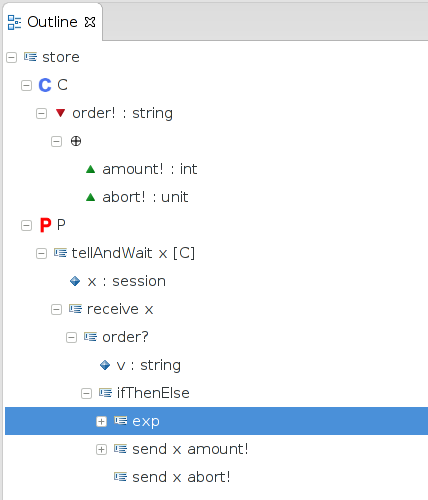
\includegraphics[scale=0.4]{img/outline.png}
    \label{fig:outline}
    \caption{caption}
  \end{figure}
}


\paragraph{Code generation and refinement.}
Diogenes translates a \coco specification
into a Java skeleton.
Considering the honest specification describe above,
Diogenes generates the following skeleton:
\begin{mdframed}
  \begin{minted}[
    fontsize=\scriptsize
    ,linenos
    ]{java}
    public class StoreHonest extends Participant { 
      public void run() {
        Session<TST> x = tellAndWait(C);           // tellAndWait x C
        
        Message msg = x.waitForReceive("order");   // receive c [ order? v:string ]
        String v = msg.getStringValue();
        
        try {
          Session<TST> y = tellAndWait(D, 10000); // tellRetract y D
          y.sendIfAllowed("req", v);
          
          try {                                   // receive y [ok? + no? + t]
            Message msg_1 = y.waitForReceive(10000, "ok", "no");
            switch (msg_1.getLabel()) {                    
              case "ok": x.sendIfAllowed("amount", 100); break;
              case "no": x.sendIfAllowed("abort"); break;                    
            }
          }
          catch (TimeExpiredException e) {        // send x abort! | receive y [ok? + no?] 
            parallel(()->{ x.sendIfAllowed("abort"); });
            parallel(()->{ y.waitForReceive("ok", "no"); });
          }            
        }
        catch(ContractExpiredException e) {
          x.sendIfAllowed("abort");               // : send x abort (line 11)
        } 
      }
    }
  \end{minted}
\end{mdframed}

\hidden{The \inlineCoco{tellRetract} corresponds to perform a tell with
  a delay (line \lineno{10}). The successive \code{waitForSession()} blocks until the delay is
  expired, throwing a \code{ContractExpiredException} if the session 
  was not fused in time (the contract has been retracted).
  The timeout \inlineCoco{t} corresponds to a \code{waitForReceived} with a timeout.
  The method blocks until a message with label \code{"ok"} or \code{"no"} is received,
  or throws a \code{TimeExpiredException} if the timeout expires.}

\bartnote{aggiungere commento su differenza tra specifica e implementazione}

% \paragraph{Refining the skeleton.}
The order amount at line \lineno{15} is still hardcoded, so we decide to separate its computation
in a separated method, \eg
\begin{mdframed}
  \begin{minted}[
    fontsize=\scriptsize
    % ,linenos
    ]{java}
    public int getOrderAmount(String order) throws MyException {...}
  \end{minted}
\end{mdframed}
and change the number \code{100} at line \lineno{15} with \code{getOrderAmount(v)}.
The method could read the order amount from a file or database,
and suppose that each possible exception
is caught and hidden behind \code{MyException}. 
The failure of this method can be considered not deterministic,
so we need to ``instruct'' our verification tool
in order to consider all the possible ways the method can terminate.
% 
To this purpose, we provide the annotation \code{@SkipMethod(value="<value>")}, that
is interpreted by the checker as follows:
\bartnote{save space}
\begin{itemize}[noitemsep,topsep=0pt]
\item ignore what the method really does. 
  This point imposes that an annotated method does not perform any action
    directed to the middleware;
\item consider \code{"<value>"} as the returning value on success;
\item consider the declared exceptions as possible exit points on failure.
\end{itemize}

Now Diogenes can symbolically consider both the case of a normal 
termination of the method
(returning the value specified in the annotation, if provided),
and all the possible exceptional terminations.

\paragraph{Verification.}
Diogenes can verify the honesty of our store 
by invoking the static method
\code{HonestyChecker.isHonest(StoreHonest.class)},
which returns one of the following values:
\begin{itemize}[noitemsep,topsep=0pt]
\item \code{HONEST}: the tool was able to extract a \coco model and verify that is honest;
\item \code{DISHONEST}: as above, but the model is dishonest;
\item \code{UNKNOWN}: the tool was unable to extract a model,
  \eg due to unhandled exceptions within the class under test.
\end{itemize}

In our example, it returns \code{UNKNOWN} and prints the following information
\begin{mdframed}
  \begin{minted}[
    fontsize=\scriptsize
    % ,linenos
    ]{java}
    error details: MyException: 
    This exception is thrown by the honesty checker. Please catch it!
    at it.unica.co2.store.Store$Phonest.getOrderAmount(Store.java:166)
    at it.unica.co2.store.Store$Phonest.run(Store.java:129)
    at it.unica.co2.honesty.HonestyChecker.runProcess(HonestyChecker.java:182)
  \end{minted}
\end{mdframed}
It means that if the method \code{getOrderAmount} will fail,
the program will be terminated abruptly and the store may be culpable.
Finally, catching \code{MyException} with \code{x.sendIfAllowed("abort")},
the program come back \emph{honest}.
\bartnote{+dettaglio}





